\subsubsection{Schwungräder}
Die Vortriebskraft für die Tennisbälle wird durch zwei Schwungräder übertragen. Die Schwungräder sind konkav ausgerundet, so dass die Beschleunigung nicht nur über einen Punkt übertragen wird. Durch die Ausrundung kann die Kraft über eine grössere Fläche (Linie) und geführt übertragen werden. Dies bringt den Vorteil, dass die Beschleunigung geführt abläuft, wodurch ein gerichteter Wurf entsteht. So kann das benötigte Beschleunigungsmoment voll umfänglich den Tennisbällen übergeben werden. Die Ausrundung wurde durch den Radius des Tennisballes gegeben. Der Durchmesser der Schwungräder ist so festgelegt, dass mit der vorhandenen Masse ein gewisses Trägheitsmoment zur Verfügung steht. Dies ist nötig, damit bei der Beschleunigung der Tennisbälle die Schwungräder nicht zu stark abgebremst werden. Dennoch sollten sie nicht zu schwer und gross sein, da das Gewicht ein wichtiger Faktor in der Gesamtbewertung ist. Die Grösse ist deshalb auf einen Kompromiss gefallen. Durch den Durchmesser wird auch die Winkelgeschwindigkeit festgelegt. Die Schwungräder sind aus PVC gefertigt. Dieser Werkstoff ist einfach zu Bearbeiten und bietet zugleich eine genügend grosse Festigkeit. Die Räder sind mit einer speziellen Haftmatte beschichtet, damit die Kraft optimal auf den Ball übertragen werden kann. \\
Die Achsen der zwei Schwungräder sind im Winkel von 45° zur Bodenplatte angeordnet. Der Abschusswinkel ist so gewählt, dass die Tennisbälle in einem genug grossen Einschlagwinkel im Zielbereich landen und keine Möglichkeit besteht mit dem Korbrand zu kollidieren. Das Verhältnis von Wurfkraft zu Wurflänge ist beim Winkel von 45° auch am besten. Die Wurfweite wird durch die Drehzahl der Schwungräder gesteuert werden. Der Achsenabstand der beiden Schwungräder bestimmt die Presskraft der einzelnen Bälle. Dies wiederum gibt die Abbremsung der Schwungräder vor. Die Abbremsung darf nicht zu gross sein, damit die einzelnen Bälle in kurzem Abstand hintereinander zugeführt werden kann. 
\begin{figure}[h!]
	\centering
	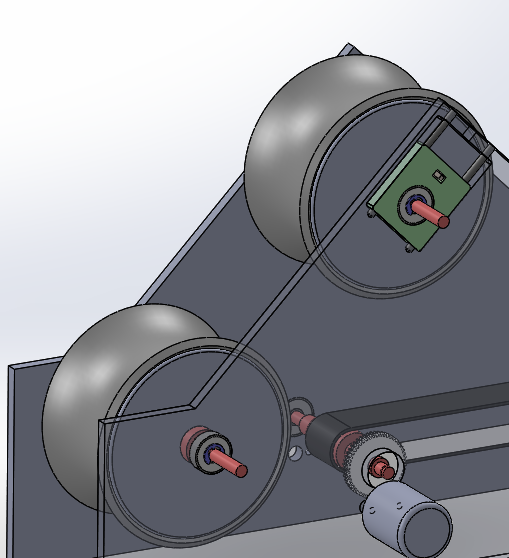
\includegraphics[width=0.9\textwidth]{Enddokumentation/Loesungskonzept/Bilder/Schwungraeder.png}
	\caption{Schwungräder}
	\label{fig:Schwungräder}	
\end{figure}
Die Schwungräder sollen aus einem Kunststoffkern sowie einem aufgeklebtem Gummielement bestehen, welches eine gewisse Nachgiebigkeit aufweist, und ein Durchrutschen der Bälle verhindern soll.  Die konkave Form der Räder gibt dem Ball die genaue Richtung der Flugbahn vor.
\paragraph{Antriebsstrang}

Der Antriebsstrang kann auf verschiedene Arten realisiert werden. Drei ausgewählte Vari-anten wurden betreffend ihrem Nutzen (verfügbares Drehmoment), ihren Kosten und ihrem Gewicht beurteilt.
\begin{figure}[h!]
	  

	\centering
  \caption{Name der Tabelle ergänzen!!!!!}
    \begin{tabular}{rrrrrr}

    \textbf{Variante} & \multicolumn{2}{r}{\textbf{beinhaltet}} & \textbf{vorh. / zul. Momente (Nutzen)} & \textbf{Preis} & \textbf{Gewicht} \\

    \multirow{9}[2]{*}{A} & 1x    & Motor & 0.1256Nm & 34.95CHF & 57.0g \\
          & 2x    & Zahnrad Z22 & 0.1256Nm / 0.33Nm & 9.62CHF & 5.1g \\
          & 2x    & Zahnrad Z90 & 0.257Nm / 4.03Nm & 3.44CHF & 57.0g \\
          & 2x    & zusätzl. Achsen & -     & 0.00CHF & 10.0g \\
          & 2x    & Kugellager & -     & 1.76CHF & 4.9g \\
          &       &       &       &       &  \\
          &       &       &       &       &  \\
          &       &       &       &       &  \\
          & \textbf{Tot.} &       & \textbf{0.257Nm} & \textbf{64.59CHF} & \textbf{211.0g} \\
    \multirow{10}[2]{*}{B} & 2x    & Motor & 0.1256Nm & 34.95CHF & 57.0g \\
          & 2x    & Zahnrad Z15 & 0.1256Nm / 0.15Nm & 2.88CHF & 2.5g \\
          & 2x    & Zahnrad Z30 & 0.257Nm / 0.68Nm & 4.05CHF & 9.4g \\
          & 2x    & Zahnrad Z15 & 0.257Nm / 0.27Nm & 3.44CHF & 3.8g \\
          & 2x    & Zahnrad Z30 & 0.514Nm / 1.24Nm & 5.50CHF & 15.0g \\
          & 4x    & Kugellager & -     & 1.76CHF & 4.9g \\
          & 2x    & zusätzl. Achsen &       & 0.00CHF & 10.0g \\
          & 2x    & Motorenaufnahme &       & 0.00CHF & 8.0g \\
          &       &       &       &       &  \\
          & \textbf{Tot.} &       & \textbf{0.514Nm} & \textbf{108.68CHF} & \textbf{201.2g} \\
    \multirow{9}[2]{*}{C} & 1x    & Motor & 0.1256Nm & 34.95CHF & 57.0g \\
          & 1x    & Zahnrad & 0.1256Nm  / 0.11Nm & 8.02CHF & 10.0g \\
          & 1x    & Zahnrad & 0.257Nm / 0.96Nm & 15.67CHF & 102.0g \\
          & 4x    & Riemenrad & 0.257Nm & 8.31CHF & 21.0g \\
          & 1x    & Riemen & 42.83N / Fzul=300N & 41.00CHF & 10.0g \\
          & 4x    & Kugellager &       & 1.76CHF & 4.9g \\
          & 3x    & Achse &       & 0.00CHF & 10g \\
          &       &       &       &       &  \\
          & \textbf{Tot.} &       & \textbf{0.257Nm} & \textbf{139.92CHF} & \textbf{312.6g} \\

    \end{tabular}%
  \label{tab:addlabel}%

\end{figure}

Aufgrund des hohen Drehmomentes und des geringen Gewichtes bei mittelmässigen Kosten, ist dies die idealste Lösung für den Antriebsstrang. Es wird ein bürstenloser Elektromotor verwendet. Die Ansteuerung des Motors ist sehr anspruchsvoll.

\paragraph{Ansteuerung und Regelung bürstenloser Motoren}
